
% !TeX document-id = {d8b4925c-2057-42a4-b894-2f1a3f1b6345}
%!TeX TXS-program:compile = txs:///xelatex/[--shell-escape]
\documentclass[aspectratio=169, mathserif]{beamer}% TPU recommends 16:9 ratio, 4:3 may require some work with inner theme .sty file

% Style options:
% light --- light theme (default)
% dark --- dark theme
% enlogo --- english TPU logo {default}
% rulogo --- russian TPU logo

\usetheme[light, rulogo]{tpu}% dark theme used as an example of optional argument

\usepackage[russian]{babel}%uncomment this to work in russian
\usepackage[utf8]{inputenc}

\usepackage{fontspec}

\setromanfont{Brygada1918}[
Path=./fonts/BrygadaFontFiles/,
Extension = .ttf,
UprightFont=*-Regular,
BoldFont=*-Bold,
ItalicFont=*-Italic,
BoldItalicFont=*-BoldItalic
]

\setsansfont{ALSSirius}[
Path=./fonts/ALSSiriusFiles/,
Extension = .otf,
UprightFont=*-Regular,
BoldFont=*-Bold,
%ItalicFont=*-Italic,
%BoldItalicFont=*-BoldItalic
]

\setmonofont{Consolas}[
Path=./fonts/ConsolasFontFiles/,
%Scale=0.85,
Extension = .ttf,
UprightFont=*-Regular,
BoldFont=*-Bold,
ItalicFont=*-Italic,
BoldItalicFont=*-BoldItalic
]

\usepackage[cache=false]{minted}
\usepackage{xcolor} % to access the named colour LightGray
\usepackage{colortbl}
\definecolor{LightGray}{gray}{0.9}
\definecolor{onedarkBckGr}{RGB}{40, 44, 52}

\usemintedstyle[python]{default}
\setminted[python]{
fontsize=\scriptsize,
escapeinside=||,
mathescape=true,
numbersep=5pt,
gobble=2,
linenos=true,
frame=leftline,
framesep=1mm,
python3=true,
%bgcolor=backcolour,
}

\usemintedstyle[pycon]{default}
\setminted[pycon]{
	fontsize=\scriptsize,
	escapeinside=||,
	mathescape=true,
	numbersep=5pt,
	gobble=2,
	frame=single,
	framesep=1mm,
	python3=true,
%	bgcolor=backcolour,
	linenos=true,
}

\newmint{python}{}

\usepackage{booktabs}% good looking tables
\usepackage{multicol}% text in multiple columns, useful for side-by-side text and pictures
\usepackage{hyperref}
\definecolor{maroon}{cmyk}{0, 0.87, 0.68, 0.32}
\definecolor{halfgray}{gray}{0.55}
\definecolor{ipython_frame}{RGB}{207, 207, 207}
\definecolor{ipython_bg}{RGB}{247, 247, 247}
\definecolor{ipython_red}{RGB}{186, 33, 33}
\definecolor{ipython_green}{RGB}{0, 128, 0}
\definecolor{ipython_cyan}{RGB}{64, 128, 128}
\definecolor{ipython_purple}{RGB}{170, 34, 255}
\definecolor{linkcolor}{HTML}{0000FF} % цвет гиперссылок
\definecolor{urlcolor}{HTML}{800080} % цвет ссылок
\definecolor{backcolour}{rgb}{0.95,0.95,0.92}

\usepackage{longtable}
\usepackage{wrapfig}
\usepackage{ragged2e}
\usepackage[nooneline]{caption}
\DeclareCaptionTextFormat{center}{\centering{#1}}
\captionsetup[table]{justification=raggedleft,
labelformat=empty,
labelsep=endash,
textformat=center,
position=top,
skip=5pt
}

\hyphenpenalty=10000% i don’t think hyphenation in presentations is a good idea, feel free to change however you like

\usepackage{chemfig}

%\includeonlyframes{c}

\title{\LARGE{Системный анализ процессов химической технологии}}
\subtitle{\textcolor{tpugreen}{\textbf{Лекция №9}} \\ \textbf{Расчет реактора изомеризации \\ легких бензиновых фракций}}
\author[]{Вячеслав Алексеевич Чузлов, \\
к.т.н., доцент ОХИ ИШПР}
\date{\today}

\begin{document}

\newcommand{\pythoninline}[1]{%
	\colorbox{white}{%
		\parbox[b][.6em]{\widthof{\mintinline[fontsize=\tiny]{ipython}{#1}}}{\mintinline[fontsize=\tiny]{ipython}{#1}}%
	}%
}

% notice usage of \titleframe and several other unconventional functions
% the reason being is custom backgrounds on these slides

\titleframe% title

%\tocframe{}% this custom frame accepts options for ToC


\subsection{Принципиальная схема}
\begin{frame}[fragile, label=c]{Принципиальная схема}
\scriptsize
\begin{figure}[h!]
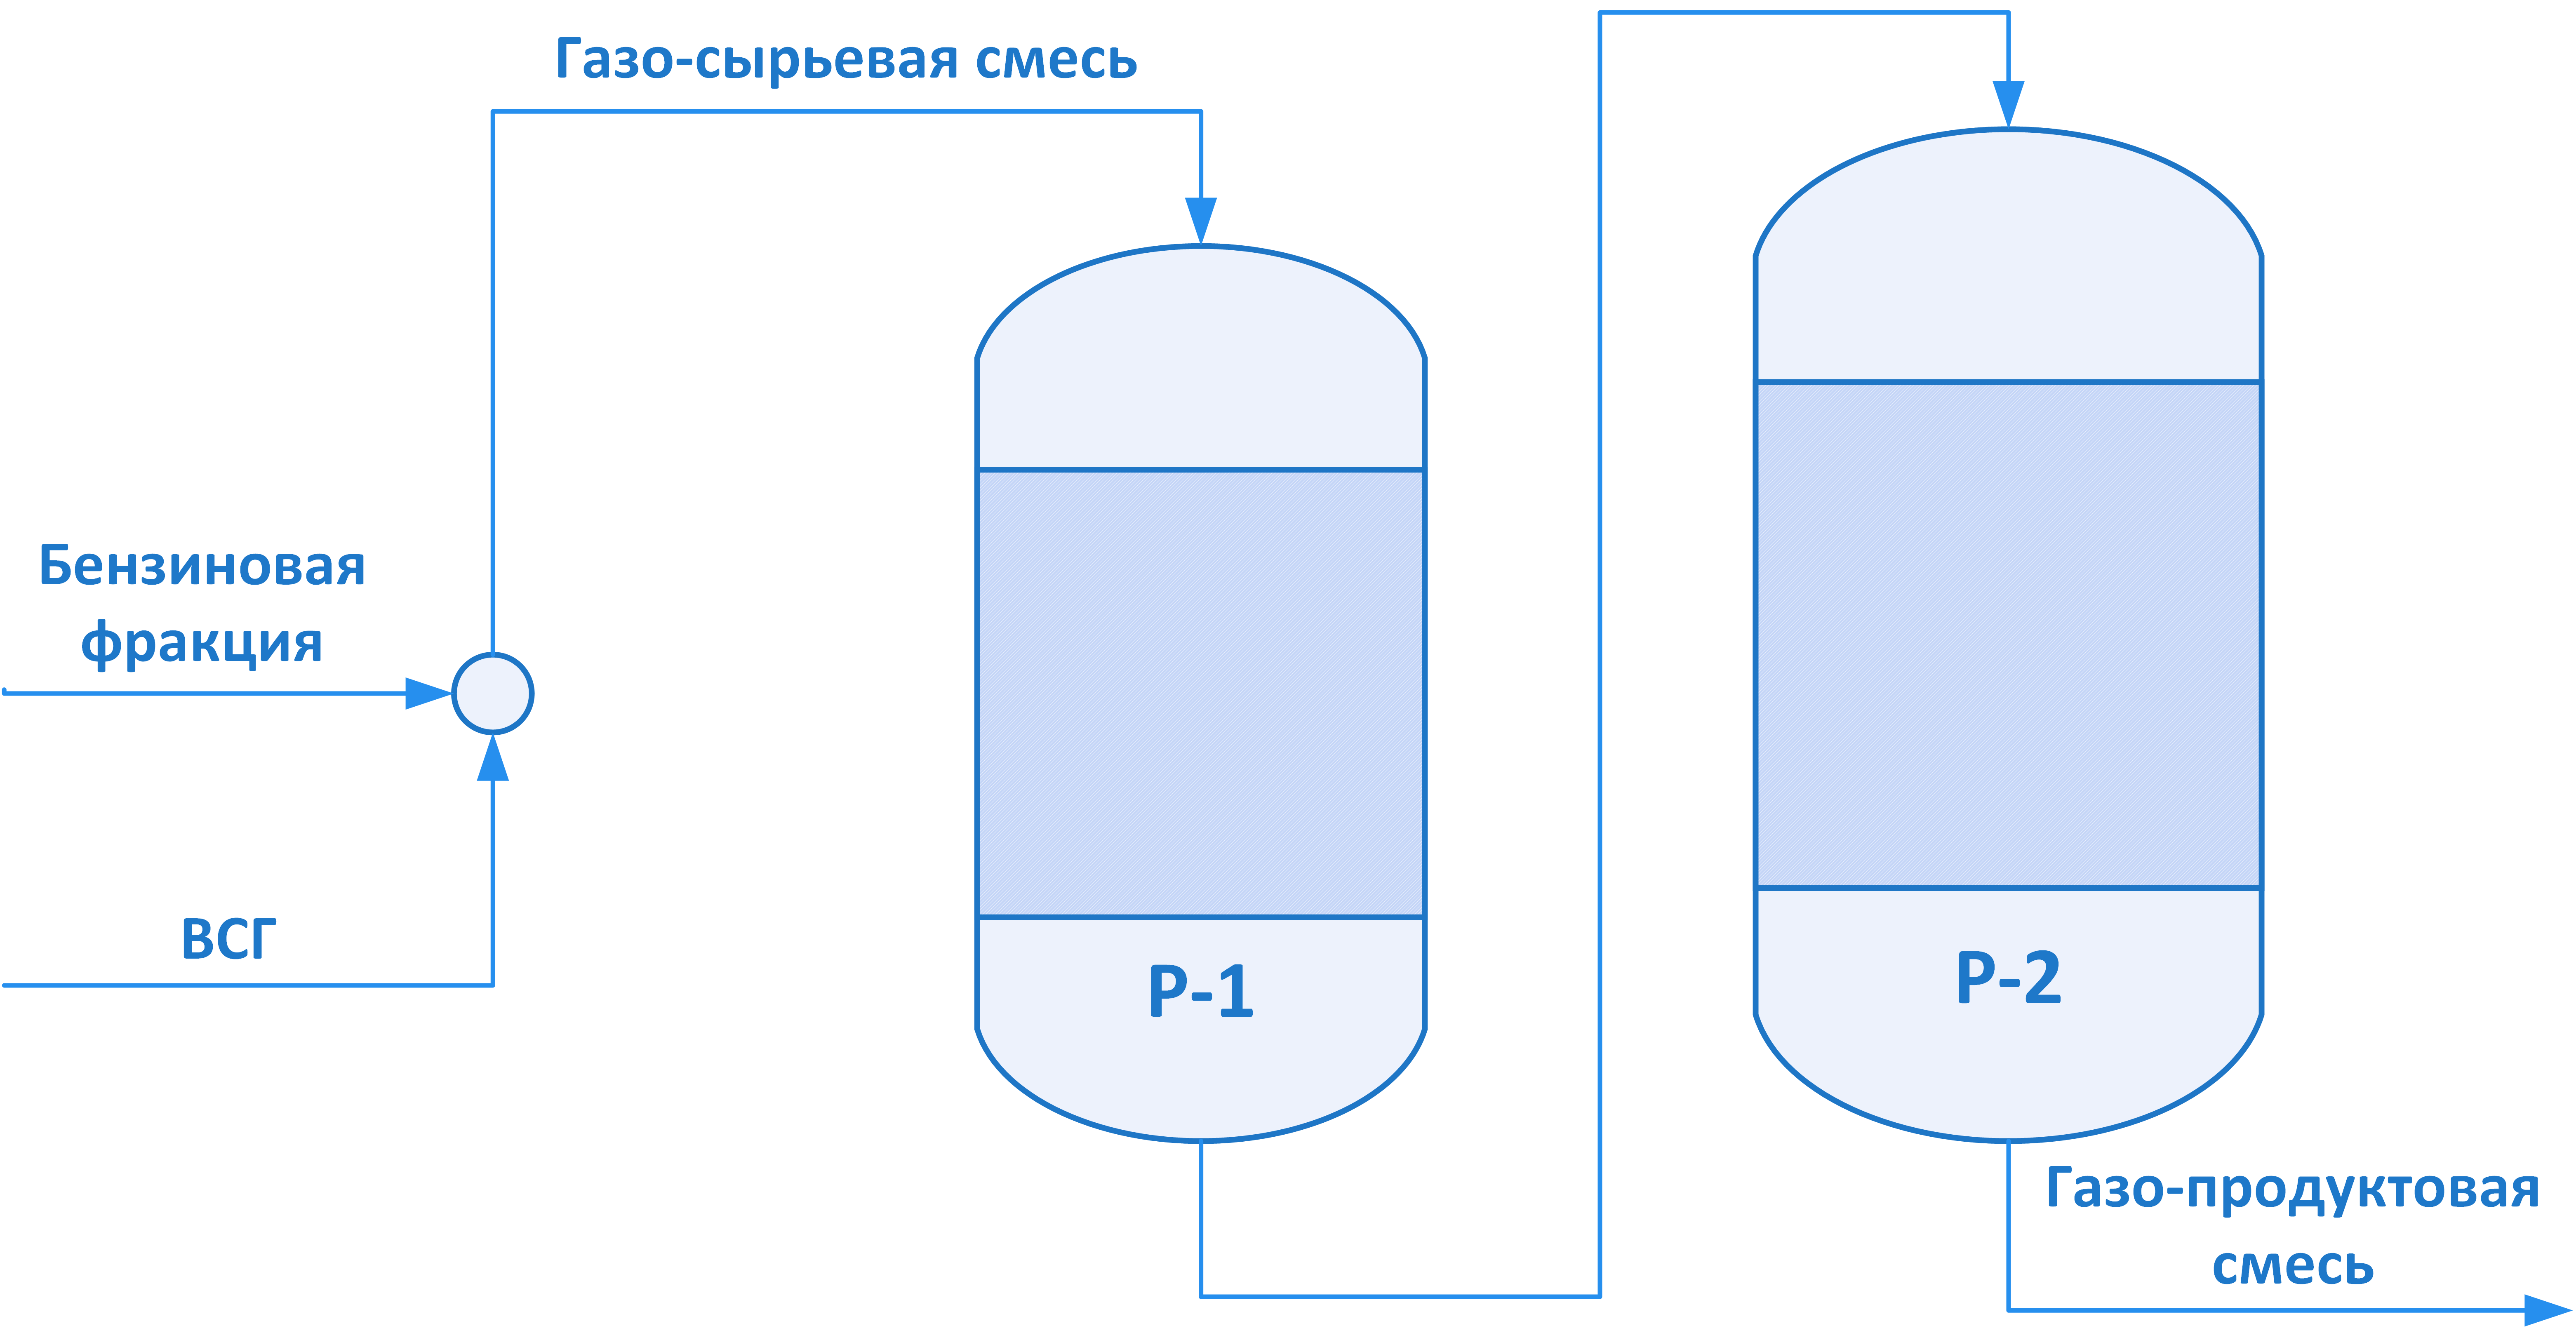
\includegraphics[width=.8\textwidth]{./pics/pfd}
\end{figure}
\vfill
\end{frame}

\subsection{Кинетическая модель процесса изомеризации}
\begin{frame}[fragile, label=c]{Кинетическая модель процесса изомеризации}
\scriptsize
\begin{figure}[h!]
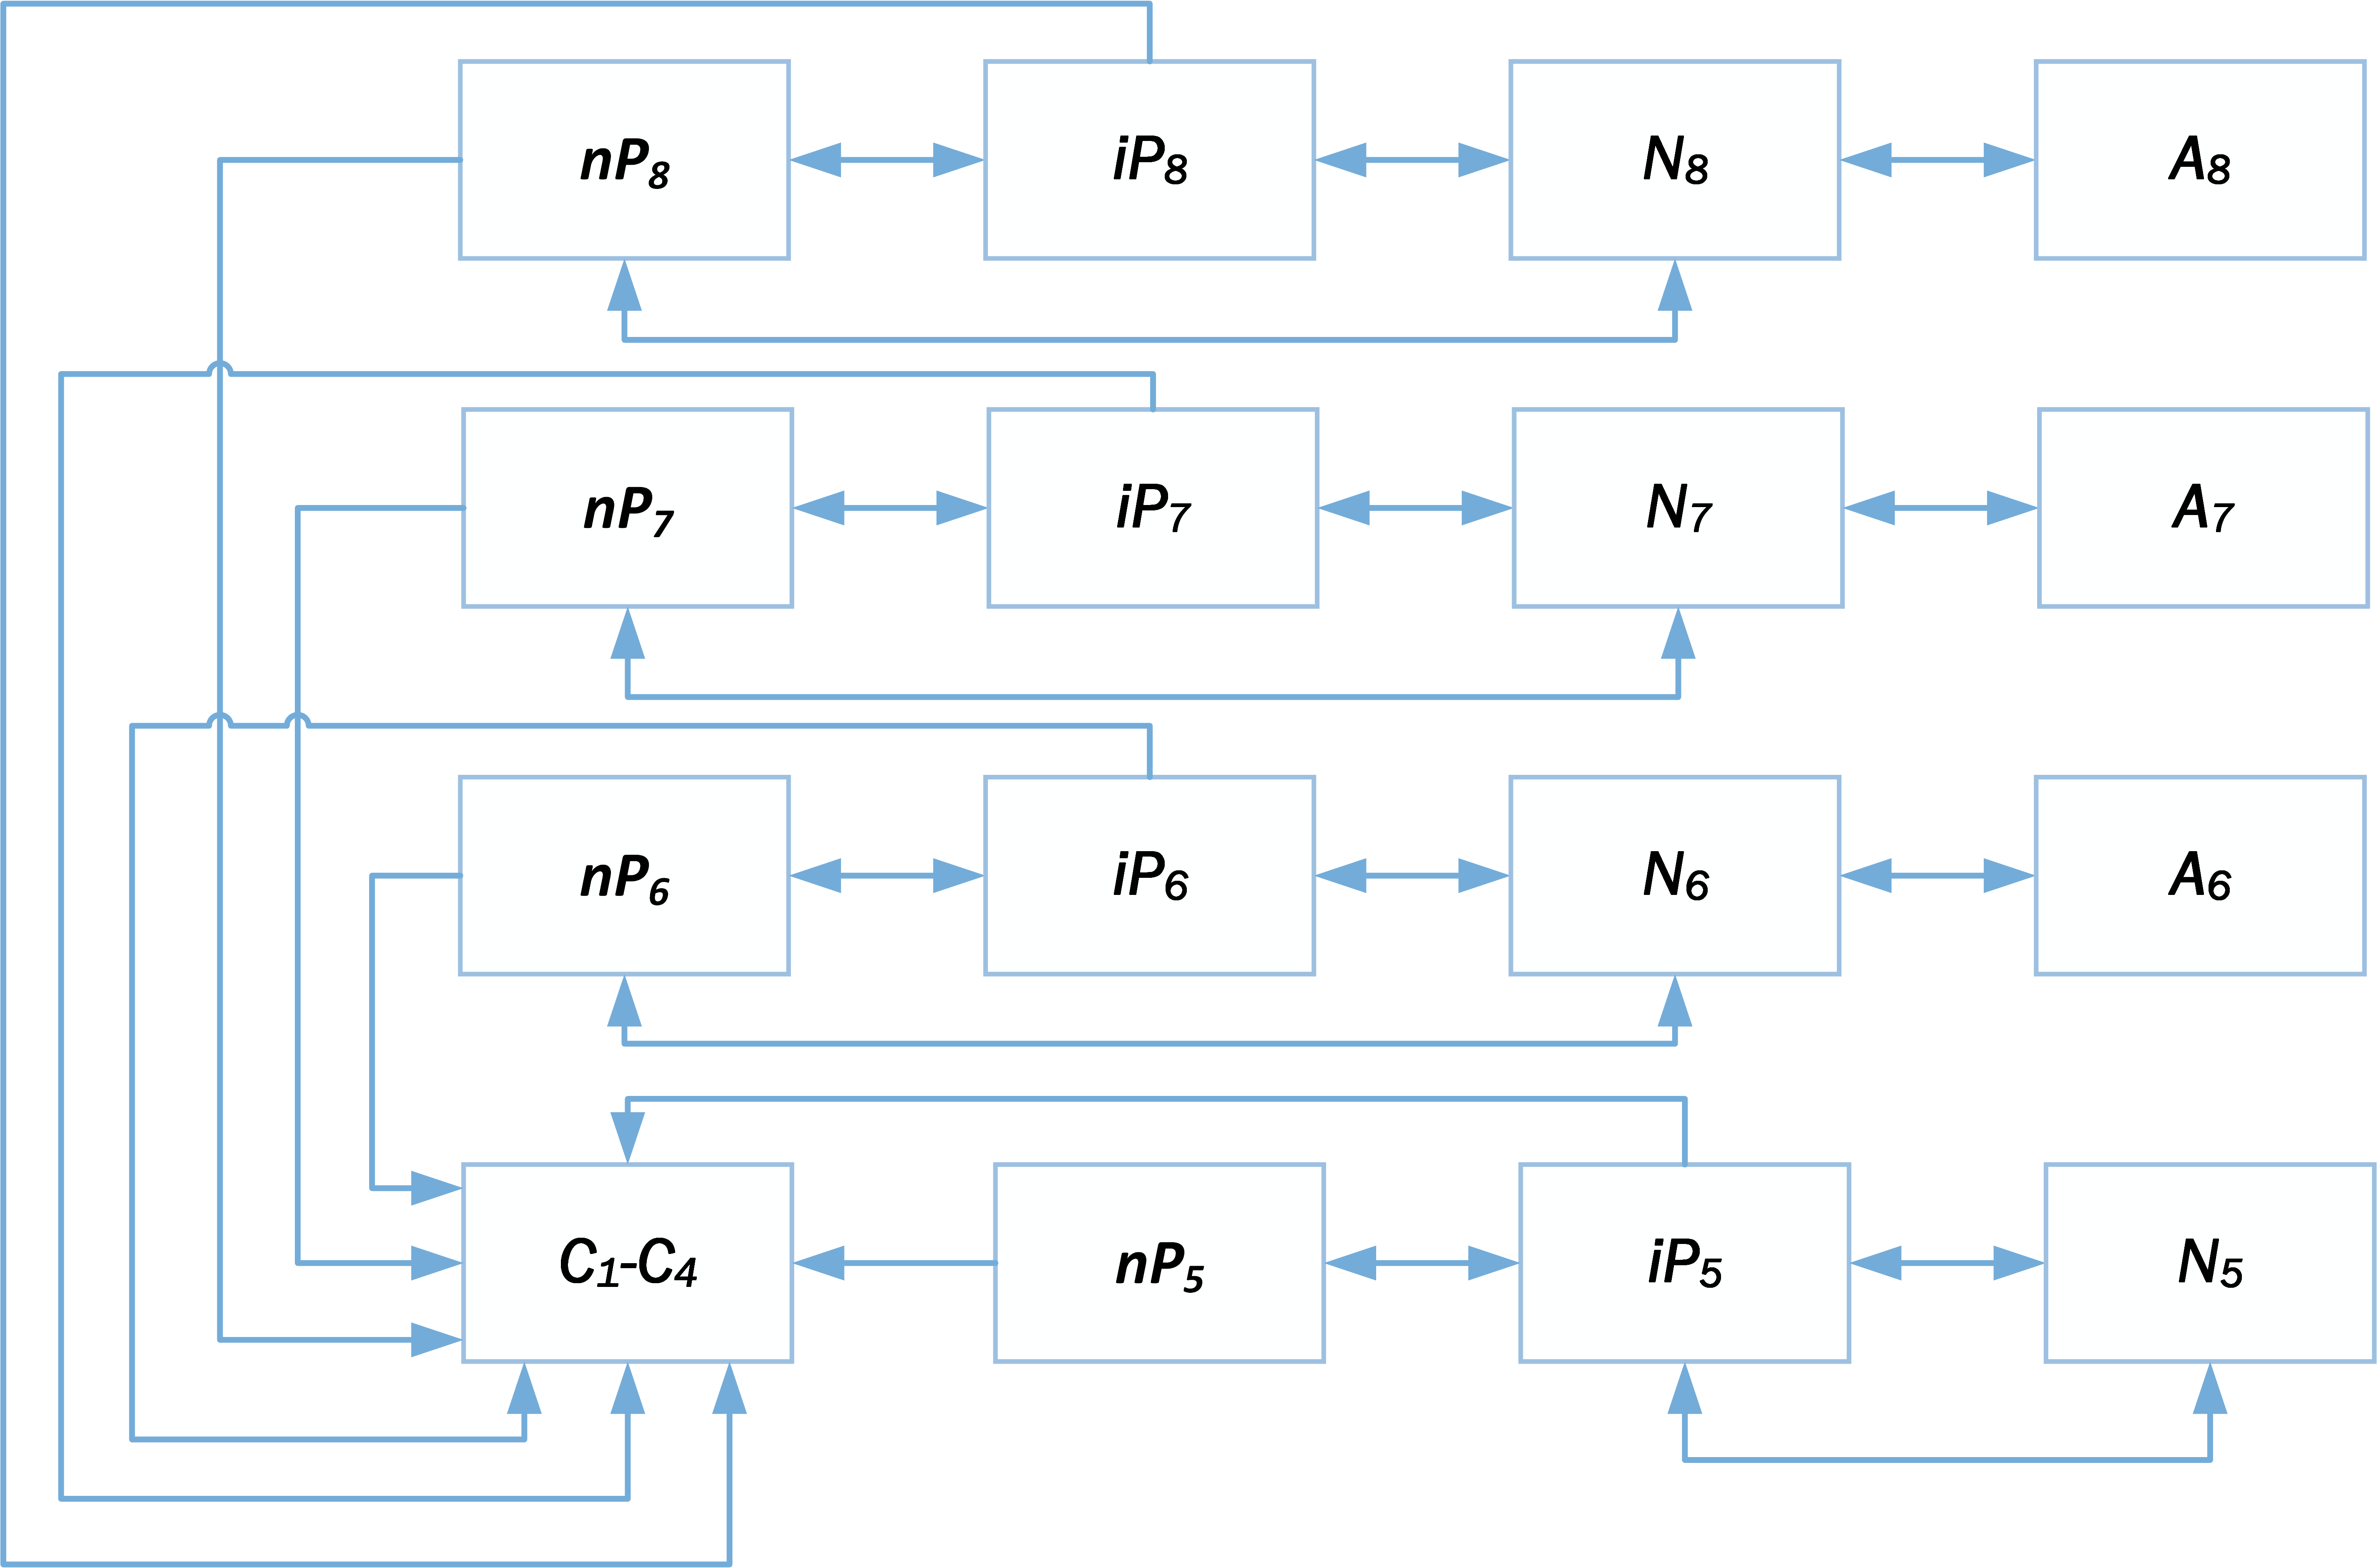
\includegraphics[width=.75\textwidth]{./pics/scheme}
\end{figure}
\vfill
\end{frame}

\subsection{Описание класса \texttt{Flow}}
\begin{frame}[fragile, label=c]{Описание класса \texttt{Flow}}
\scriptsize
\begin{table}[h!]
	\centering
	\renewcommand{\arraystretch}{1.2}
	\begin{tabular}{|p{.49\linewidth}|p{.49\linewidth}|}
		\hline
		\textbf{Атрибуты класса} & \textbf{Описание}  \\
		\hline
		\mintinline{python}|mass_flow_rate: float| & Массовый расход, кг / ч \\
		\hline
		\mintinline{python}|mole_flow_rate: float| & Мольный расход, кмоль / ч \\
		\hline
		\mintinline{python}|volume_flow_rate: float| & Объемный расход, м$^3$ / ч \\
		\hline
		\mintinline{python}|mass_fractions: np.ndarray| & Массовые доли \\
		\hline
		\mintinline{python}|mole_fractions: np.ndarray| & Мольные доли \\
		\hline
		\cellcolor{blue!25} \mintinline{python}|molar_fractions: np.ndarray| & \cellcolor{blue!25} Молярная концентрация, моль / л \\
		\hline
		\mintinline{python}|volume_fractions: np.ndarray| & Объемные доли \\
		\hline
		\mintinline{python}|temperature: float| & Температура потока, К \\
		\hline
		\cellcolor{blue!25} \mintinline{python}|pressure: float| & \cellcolor{blue!25} Давление потока, кПа \\
		\hline
		\mintinline{python}|density: float| & Плотность потока, г / см$^3$ \\
		\hline
		\cellcolor{blue!25} \mintinline{python}|ideal_gas_density: float| & \cellcolor{blue!25} Плотность потока для идеального газа, кг / м$^3$ \\
		\hline
		\mintinline{python}|average_mol_mass: float| & Средняя молекулярная масса потока, г / моль \\
		\hline
		\mintinline{python}|cp: float| & Массовая теплоемкость потока, кДж / кг \\
		\hline
%\begin{minipage}{\linewidth}
%\begin{minted}[frame=none, linenos=false]{python}
%def __init__(
%    self,
%    mass_flow_rate: float,
%    mass_fractions: np.ndarray,
%    temperature: float
%) -> None
%\end{minted}
%\end{minipage}
%		& Создает новый экземпляр класса \texttt{Flow}, заполняя все поля \\
%		\hline
	\end{tabular}
\end{table}
\vfill
\end{frame}

\begin{frame}[fragile, label=c]{Описание класса \texttt{Flow}}
\scriptsize
\begin{table}[h!]
	\centering
	\renewcommand{\arraystretch}{1.2}
	\begin{tabular}{|p{.49\linewidth}|p{.49\linewidth}|}
		\hline
		\textbf{Атрибуты класса} & \textbf{Описание}  \\
		\hline
\begin{minipage}{\linewidth}
\begin{minted}[frame=none, linenos=false]{python}
def __init__(
    self,
    mass_flow_rate: float,
    mass_fractions: np.ndarray,
    temperature: float,
    pressure: float
) -> None
\end{minted}
\end{minipage}
		&
\begin{minipage}{\linewidth}
Создает новый экземпляр класса \texttt{Flow}, заполняя все поля
\end{minipage}
 \\
		\hline
	\end{tabular}
\end{table}
\vfill
\end{frame}

\subsection{Функции для пересчета составов}
\begin{frame}[fragile, label=c]{Функции для пересчета составов}
\scriptsize
\begin{enumerate}
\item Пересчет массовых долей в молярные концентрации (моль / л):
\vfill
\begin{equation*}
	c _i = \dfrac{\omega _i \cdot \rho}{M_i}
\end{equation*}
\vfill
где $c _i$~-- молярная концентрация $i$-го компонента (моль / л); $\omega _i$~-- массовая доля $i$-го компонента; $\rho $~-- плотность потока для идеального газа (кг / м$^3$); $M _i$~-- молярная масса $i$-го компонента; $i$~-- индекс компонента в системе.
\vfill
\item Пересчет молярных концентраций в массовые доли:
\vfill
$$
	\rho = \sum \limits _{i=1} ^{n} c_i \cdot M_i \qquad \omega _i = \dfrac{c_i \cdot M_i}{\rho}
$$
\vfill
где $\omega _i$~-- массовая доля $i$-го компонента; $c _i$~-- молярная концентрация $i$-го компонента (моль / л); $\rho $~-- плотность потока для идеального газа (кг / м$^3$); $M_i$~-- молярная масса $i$-го компонента; $n$~-- число компонентов в системе; $i$~-- индекс компонента в системе.
\vfill
\end{enumerate}
\vfill
\end{frame}


\subsection{Функции для расчета плотности идеального газа}
\begin{frame}[fragile, label=c]{Функции для расчета плотности идеального газа}
\scriptsize
Расчет плотности идеального газа:
\vfill
\begin{equation*}
	\rho = \dfrac{p \cdot M}{R \cdot T}
\end{equation*}
\vfill
где $\rho$~-- плотность потока (кг / м$^3$); $p$~-- давление потока, кПа; $M$~-- средняя молекулярная масса потока, кг / моль; $R$~-- универсальная газовая постоянная, $8.314$ Дж / (моль $\cdot$ К); $T$~-- температура потока, К.
\vfill
\end{frame}


\subsection{Описание класса \texttt{Bed}}
\begin{frame}[fragile, label=c]{Описание класса \texttt{Bed}}
\scriptsize
\begin{table}[h!]
\centering
\renewcommand{\arraystretch}{1.2}
\begin{tabular}{|p{.49\linewidth}|p{.49\linewidth}|}
	\hline
	\textbf{Атрибуты класса} & \textbf{Описание}  \\
	\hline
\begin{minipage}{\linewidth}
\vfill
\begin{minted}[frame=none, linenos=false]{python}
def __init__(
        self,
        diameter: float = None,
        height: float = None,
        volume: float = None
) -> None
\end{minted}
\vfill
\end{minipage}
	&
\begin{minipage}{\linewidth}
Конструктор класса, необходимо передать диаметр и высоту, диаметр и объем или высоту и объем полки
\end{minipage}
\\
	\hline
\begin{minipage}{\linewidth}
\vfill
\begin{minted}[frame=none, linenos=false]{python}
def __repr__(self) -> str
\end{minted}
\vfill
\end{minipage}
		& Строковое представление объекта класса \texttt{Bed} \\
		\hline
\begin{minipage}{\linewidth}
\vfill
\begin{minted}[frame=none, linenos=false]{python}
def calculate(
    self,
    kinetic_scheme: callable,
    feedstock: Flow,
    ea: np.ndarray,
    predexp: np.ndarray
) -> Flow
\end{minted}
\vfill
\end{minipage}
		&
\begin{minipage}{\linewidth}
Расчет системы дифференциальных уравнений изменения концентрации компонентов по времени
\end{minipage}
\\
		\hline
	\end{tabular}
\end{table}
\vfill
\end{frame}


\subsection{Описание класса \texttt{Reactor}}
\begin{frame}[fragile, label=c]{Описание класса \texttt{Reactor}}
\scriptsize
\begin{table}[h!]
\centering
\renewcommand{\arraystretch}{1.2}
\begin{tabular}{|p{.49\linewidth}|p{.49\linewidth}|}
	\hline
	\textbf{Атрибуты класса} & \textbf{Описание}  \\
	\hline
\begin{minipage}{\linewidth}
\vfill
\begin{minted}[frame=none, linenos=false]{python}
def __init__(
    self,
    *bed_params: dict
) -> None
\end{minted}
\vfill
\end{minipage}
	&
\begin{minipage}{\linewidth}
Конструктор класса, необходимо передать диаметр и высоту, диаметр и объем или высоту и объем для каждой полки в виде словаря
\end{minipage}
	\\
	\hline
\begin{minipage}{\linewidth}
\vfill
\begin{minted}[frame=none, linenos=false]{python}
def calculate(
    self,
    kinetic_scheme: callable,
    feedstock: Flow,
    ea: np.ndarray = const.EA,
    predexp: np.ndarray = const.PREDEXP
) -> Flow
\end{minted}
\vfill
\end{minipage}
		&
\begin{minipage}{\linewidth}
Расчет системы дифференциальных уравнений изменения концентрации компонентов по времени для каждой полки катализатора
\end{minipage}
		\\
		\hline
\begin{minipage}{\linewidth}
\vfill
\begin{minted}[frame=none, linenos=false]{python}
def performance(self) -> dict
\end{minted}
\vfill
\end{minipage}
		& Метод, возвращающий словарь с информацией об эффективности процесса изомеризации: выход изомеризата, выход изоалканов \\
		\hline
	\end{tabular}
\end{table}
\vfill
\end{frame}


\subsection{Расчет кинетических параметров}
\begin{frame}[fragile, label=c]{Расчет кинетических параметров}
\scriptsize
\begin{minipage}{.6\textwidth}
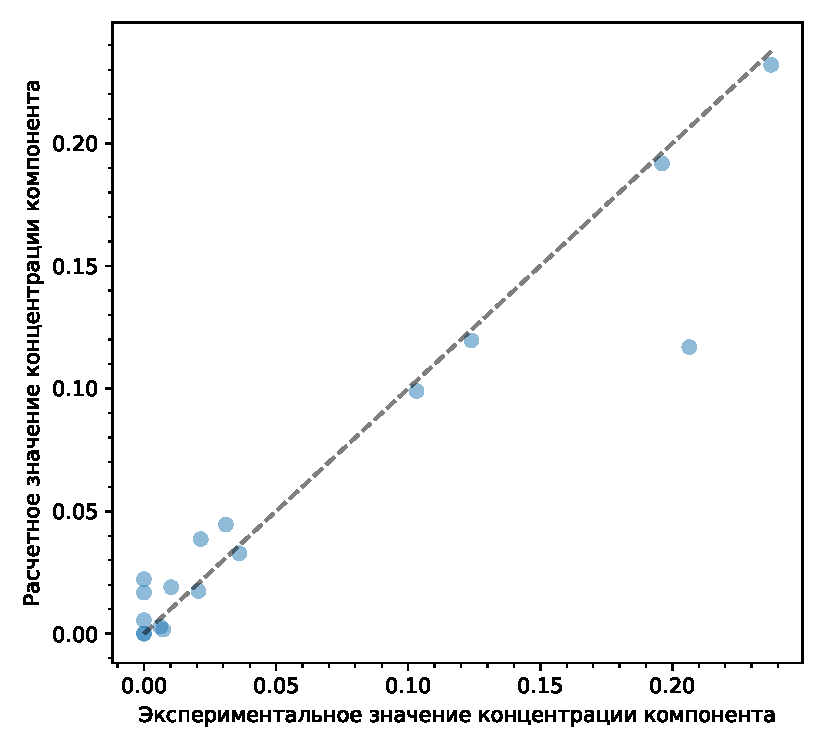
\includegraphics[width=\linewidth]{./pics/err}
\end{minipage}
\begin{minipage}{.39\textwidth}
\begin{itemize}
\item Обратная кинетическая задача была решена методом Нелдера-Мида с ограничением по минимальному значению констант: \mintinline{python}|(0, None)|;
\item Оптимизируемая функция:
\vfill
$$
	error = \sum \limits _{i=1} ^{n} \left(c_i - c_{i, calc}\right) ^2
$$
\vfill
\item Значение $error = 0.009515497205293953$.
\end{itemize}
\vfill
\end{minipage}
\vfill
\end{frame}



\contactsframe[\Large \textbf{Благодарю за внимание!}]{


\includegraphics[width=.05\textwidth]{pics/home} \quad Учебный корпус №2, ауд. 136 \\

\includegraphics[width=.05\textwidth]{pics/mail} \quad chuva@tpu.ru \\

\includegraphics[width=.03\textwidth]{pics/tel} \quad +7-962-782-66-15
}

\end{document}

